%\documentclass[10pt,handout]{beamer}
\documentclass[10pt]{beamer}
\usepackage{babel} % Anpassa efter svenska. Ger svensk logga.
\usepackage[utf8]{inputenc} % Anpassa efter linux
\usepackage{graphicx}
\usepackage{../common/beamerthemeUppsala}
%\usecolortheme{UU} % Anpassa efter UU:s frger och logga
%\hypersetup{pdfpagemode=FullScreen} % Adobe Reader ska ppna fullskrm
\setbeamertemplate{itemize items}[circle]

% \usepackage{beamerthemesplit}
\usepackage{amsmath}
\usepackage{amssymb}
% \usepackage{graphics}
% \usepackage{graphicx}
% \usepackage{epsfig}
% \usepackage[latin1]{inputenc}
 \usepackage{color}
% \usepackage{fancybox}
% \usepackage{psfrag}
% \usepackage[english]{babel}
 \setbeamertemplate{footline}{\hfill\insertframenumber/\inserttotalframenumber}


% Read in commands
% Course settings
\newcommand{\currentsemester}{Autumn 2024}

% New commands
\newcommand{\bfm}[1]   {\mbox{\boldmath{${#1}$}}}
\newcommand{\Prob}   {\mbox{\textnormal{P}}}
\newcommand{\uured}[1]{\textcolor{uured}{#1}}

% Eqds
\def\eqd{\,{\buildrel d \over =}\,}

% Math operators
\DeclareMathOperator{\E}{\mathbb{E}}
\DeclareMathOperator{\V}{\mathbb{V}}



%%%%%%%%%%%%%%%%%%%%%%%%%%%%%%%%%%%%%%%%%%%%%%%%%%%%%%%%%%%%%%%%%%

\setlength{\parskip}{3mm}
\title[]{{\color{black}Machine learning -- Large Language Models}}
\author[]{M{\aa}ns Magnusson\\Department of Statistics, Uppsala University}
\date{\currentsemester}


\begin{document}

\frame{\titlepage
% \thispagestyle{empty}
}

%%%%%%%%%%%%%%%%%%%%%%%%%%%%%%%%%%%%%%%%%%%%%%%%%%%%%%%%%%%%%%%%%%




\section{Introduction} % to Large Language Models

\begin{frame}{What is a Large Language Model?}

\begin{itemize}
  \item Large Language Models (LLM) are commonly defined as:
  \begin{itemize}
      \item large natural language models (usually transformer-based)
      \pause
      \item generative and autoregressive, predicting a token at a time, based on previous \uured{context}
      \pause
      \item having some ability to achieve \uured{general-purpose language "understanding"}
      \item show \uured{emergent} abilities to solve other more complex tasks
      \pause
      \item fit for few-shot learning and \uured{incontext} learning
      \pause
      \item pre-trained on very large data
  \end{itemize}
  \item Compared to pretrained language models (PLM), LLMs are
  \begin{itemize}
      \item larger (billions or trillions, rather than millions of parameters), in practice only possible to train by a few persons
      \item possible to use for in-context learning
      \item usually interacted with through the prompt
  \end{itemize}
\end{itemize}

\end{frame}

\begin{frame}{Historical development}

\begin{figure}[h]
\centering
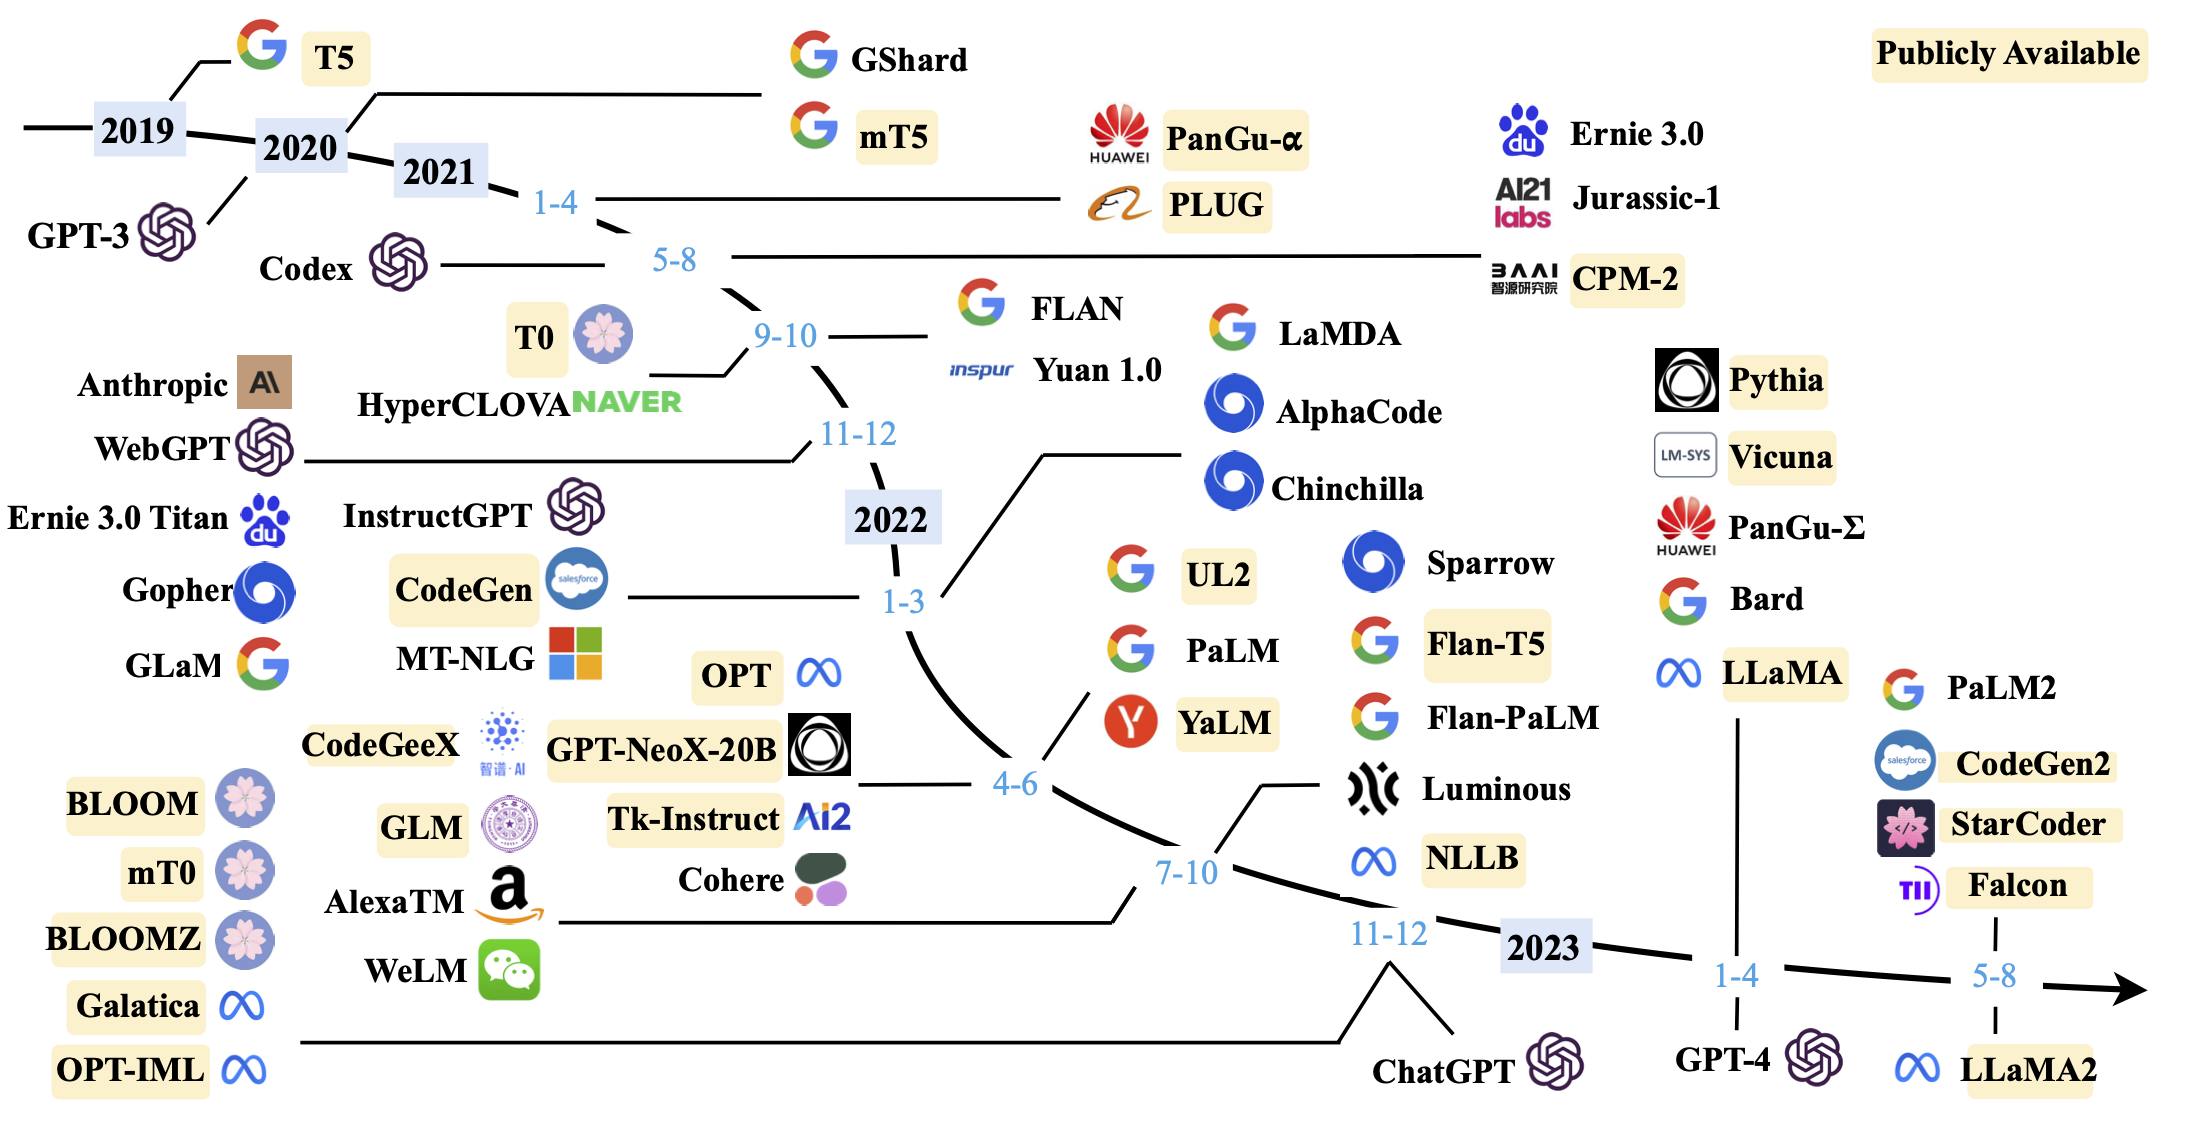
\includegraphics[width=0.99\textwidth]{fig/fig2_zhao_2023}
\caption{The development of LLMs (Figure 2, Zhao et al., 2023)}
\end{figure}

\begin{itemize}
    \item Milestones (subjective): GPT-3, GPT-4, chatGPT, Llama 2
\end{itemize}

\end{frame}

\begin{frame}{A subset of current LLMs}

\begin{figure}[h]
\centering
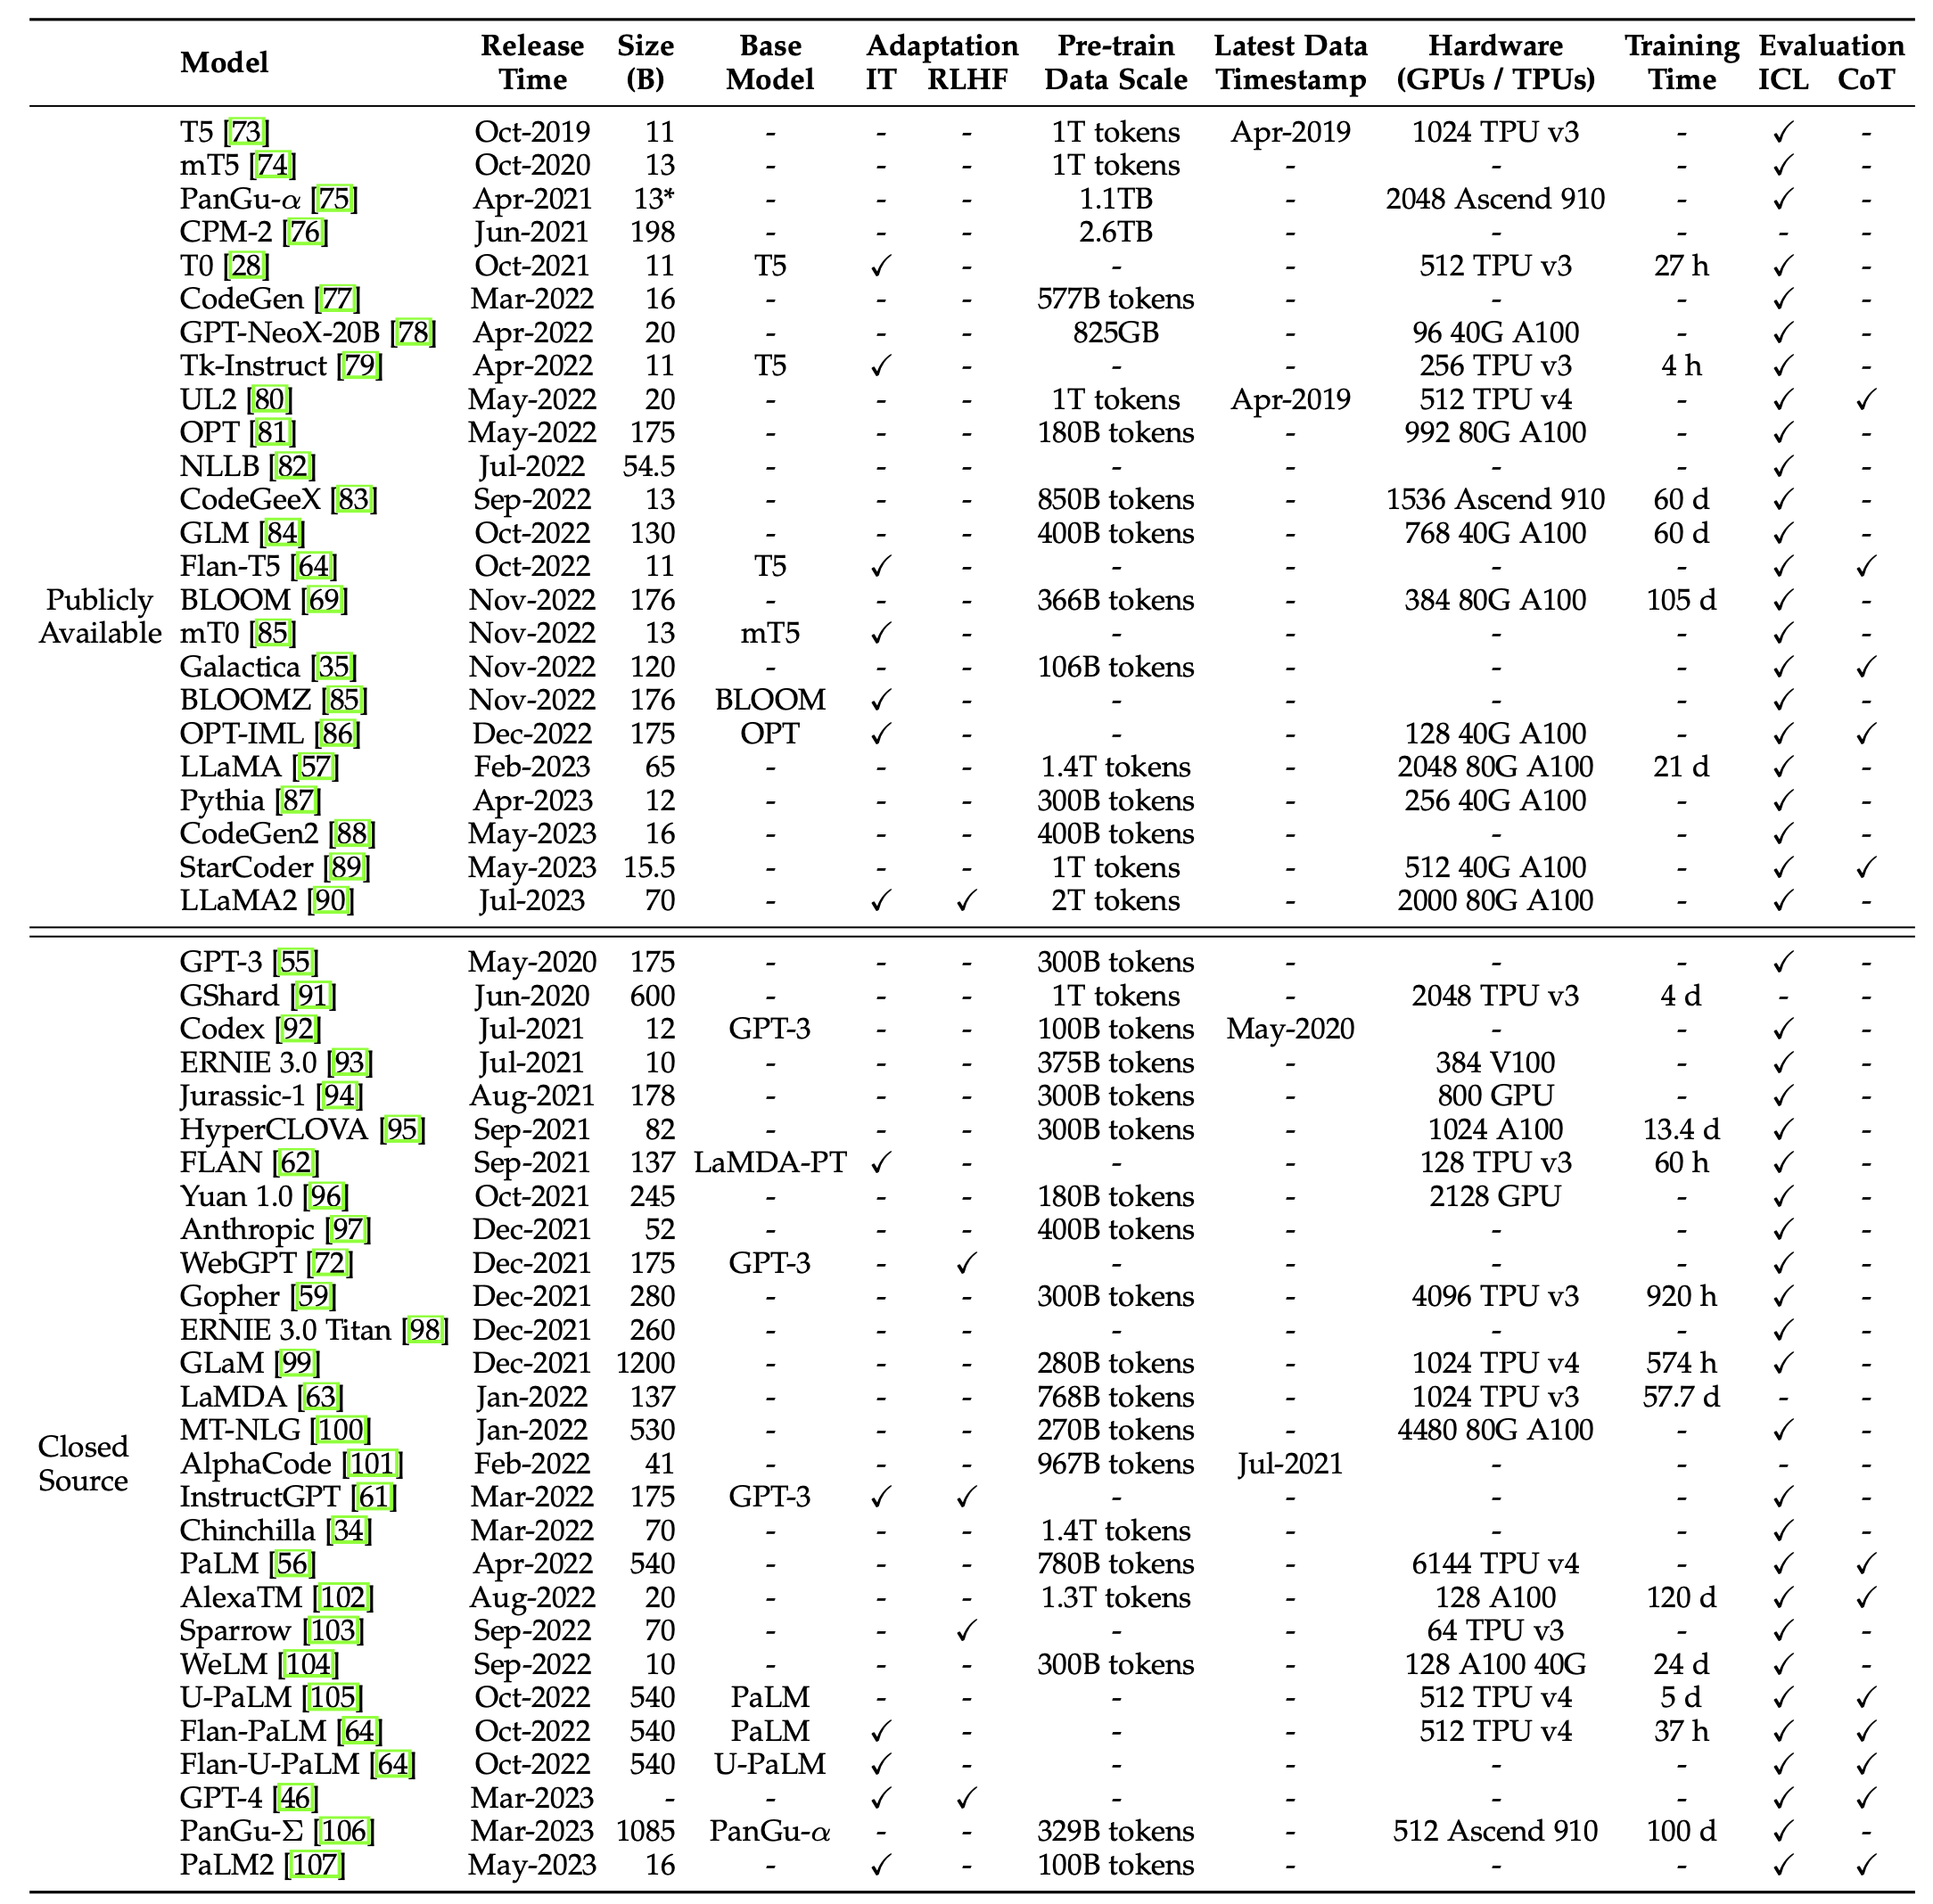
\includegraphics[width=0.82\textwidth]{fig/tab1_zhao_2023}
\caption{Statistics of LLMs (Table 1, Zhao et al., 2023)}
\end{figure}

\end{frame}

\begin{frame}{Examples of LLM prompting}

Examples:
\begin{enumerate}
\item Can you please add 113329 and 719292? (true is 832621)
\item Who is Olof Palme? Please respond both in English and Swedish.
\end{enumerate}

\centering

\vspace{5mm}

\href{https://www.llama2.ai/}{Llama 2}

\vspace{10mm}

\href{https://chat.openai.com/}{chatGPT}

\end{frame}


\begin{frame}{Why is this working now?}

\begin{itemize}
\item Scaling of pretrained models, performals (loss) improves by:
\begin{itemize}
\item Larger models (GPT3 175B, PaLM 540B)
\item Larger datasets
\item More computation
\item Scaling laws (CITE, CITE) show that all three are important\\
\uured{Can we connect this back to the standard ML framework?}
% Scaling laws has shown that all three matters and is of importance.
\end{itemize}
\pause
\item Fine-tuning for tuning models to follow instructions (InstructGPT)
\end{itemize}

\end{frame}


%\begin{frame}{Scaling laws}

%Extensive research has shown that scaling can largely improve the model capacity of LLMs

% Scale Matters/ Scaling laws p 4 in Zhao
% model performance with respective to three major factors
% namely model size (N), dataset size (D),

%\end{frame}


\begin{frame}{Emergant abilities}
% Emergent abilities
% p 4 in Zhao
\begin{itemize}
\item "the abilities that are not present in small models but arise in large models" (Zhao et al, 2023)
\item One of the main differences between LLMs and PLMs
\item Examples:
\begin{itemize}
\item In-context learning (basis for prompting)
\item Instruction following % "LaMDA-PT started to significantly outperform the untuned one on unseen tasks when the model size reached 68B, but not for 8B or smaller model sizes."
\item Step-by-step reasoning
\end{itemize}
\end{itemize}



\end{frame}


\begin{frame}{In-context learning (ICL)}

\begin{itemize}
\item Learning tasks in the actual context (think chat).
\item We demonstrate what to do with a few examples
\item The model learn what todo \uured{in context}
\item ICL only prompts LLMs for utilization
\item Let
\[
D_k = \left(f(x_1, y_1),...,f(x_k, y_k) \right)
\]
then
\[
\hat{y} = \text{LLM}(I, \underbrace{\left(f(x_1, y_1),...,f(x_k, y_k)\right)}_{demonstrations}, \underbrace{f(x_{k+1}}_{input} , ...)
\]
where $I$ is the general instructions.
\item The problem is to design the instructions in a good way.
\item What happens under the hood? We position the model in embeddings space.
\item Crazy examples: "Take a deep breath and think hard."
\item Several studies have shown that the effectiveness of ICL is highly affected by the design of demonstrations %[350, 370, 371]

\end{itemize}

% TODO: A comprehensive review of ICL has been presented in the survey paper [50], and we suggest the readers refer- ring to it for a more general, detailed discussion on this topic.
% In-context learning
% 6.1 Zhao

\end{frame}


\begin{frame}{Demonstration}
% Zhao see 6.1.2.
% the selected demon- stration examples in ICL should contain sufficient informa- tion about the task to solve as well as be relevant to the test query, for the above two selection approaches.

\begin{itemize}
\item  Demonstration selection
\begin{itemize}
\item Not well explored: k-NN based retriever to select examples
\item To resolve this issue, diversity-based selection strategies are proposed to choose the most representative set of examples for specific tasks
\item LLM-based methods to choose examples. E.g. ome recent studies employ LLM itself as the demonstration generator without human intervention
\end{itemize}
\item Demonstration format
\begin{itemize}
\item "Lets think step by step", "Take a deep breath and think."
\end{itemize}
\item Demonstration order
\begin{itemize}
\item Indications of recency bias (they are prone to repeat answers that are near the end of demonstrations)
\item Why?
\end{itemize}

\end{itemize}


\end{frame}




\begin{frame}{Chain of thought (CoT) prompting}

% Zhao Section 6.2

\begin{itemize}
\item Prompting strategy to improve performance in "reasoning"
\item Incorporates intermediate reasoning steps that can lead to the final output
\item instead of (input, output), we use (input, cot, output)
\item Zero-shot CoT: "Lets think step by step"
\end{itemize}

\begin{figure}[h]
\centering
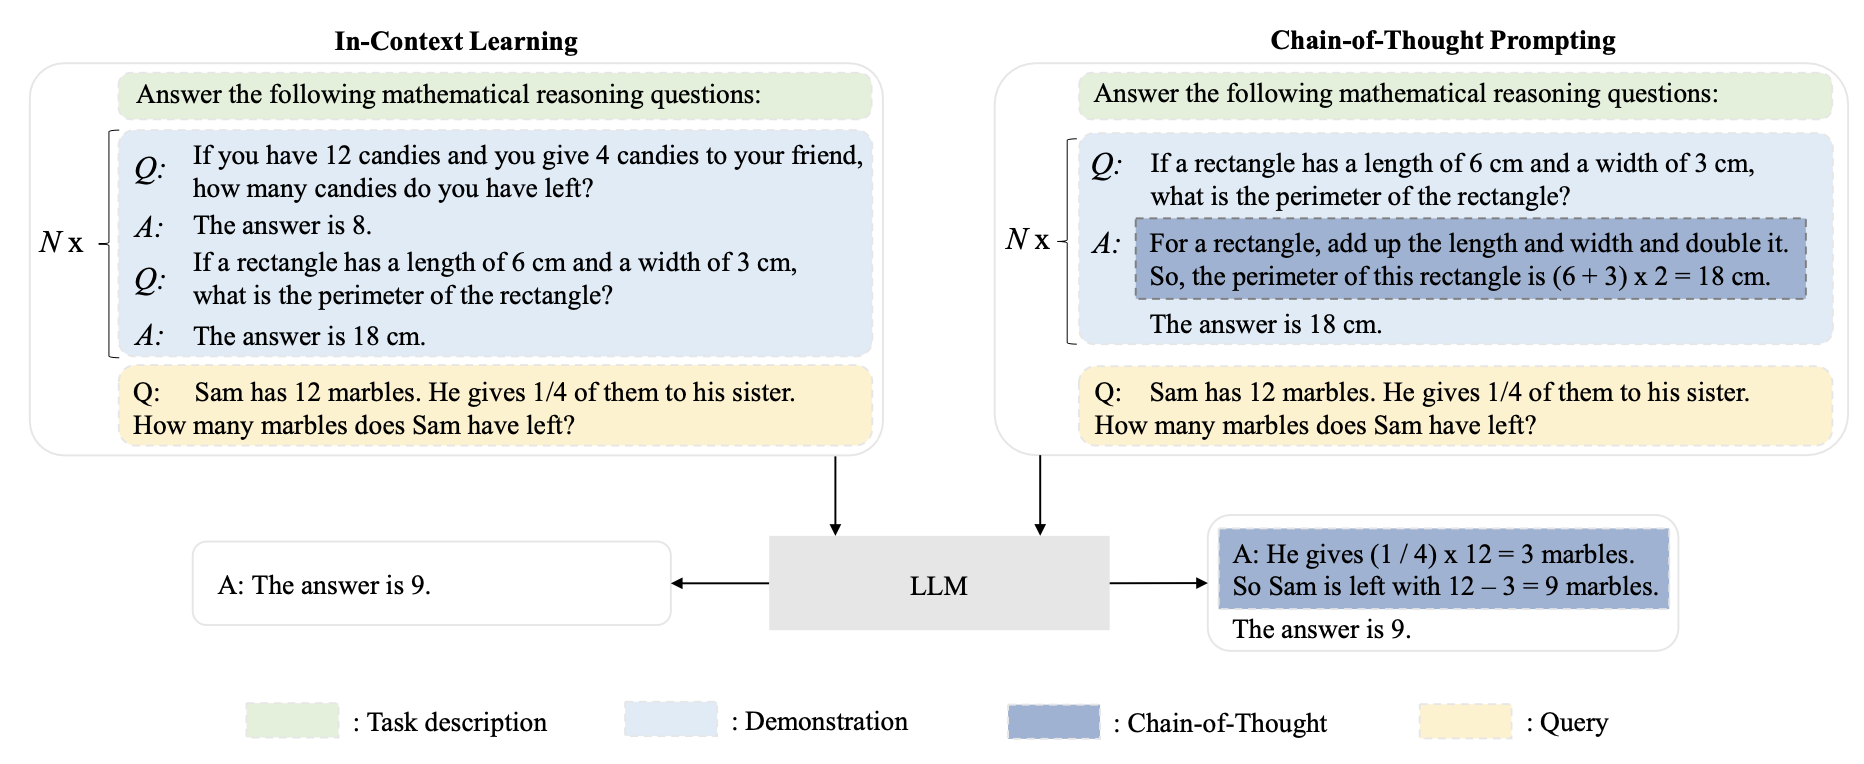
\includegraphics[width=0.99\textwidth]{fig/zhao_2023_fig12}
\caption{ICL vs CoT (Figure 12, Zhao et al., 2023)}
\end{figure}

\end{frame}

\begin{frame}{Instruction tuning/following}

% instruction tuning (discussed in Section 5.1)
\begin{itemize}
\item instruction tuning is the approach to fine-tuning pre-trained LLMs on a collection of formatted instances
\item Generally, an instruction-formatted instance consists of a task description (called an instruction), an optional input, the corresponding output, and a small number of demon- strations (optional).
\item For instruction tuning, there are two kinds of important instruction data, namely task-formatted instructions and daily chat instructions.
\item There are multiple ways to create (supervised) data, manual (NLP datasets), using API interactions, creating synthetic data
\item In- struction tuning is an effective approach to adapting existing general LLMs to be domain-specific experts. For instance, researchers propose to fine-tune Flan-PaLM [64] using medi- cal datasets to create Med-PaLM [282], a medical knowledge assistant that achieves performance levels comparable to those of expert clinicians.
\item Key crucial aspects:
\begin{itemize}
\item Scaling - a large number of instances, but the effect is descreasing
\item Including things to avoid, reasons, and suggestions, into instructions may have a negligible or even adverse effect on the performance of LLMs
\item To summarize: diversity and quality of instructions seem to be more important than the number of instances
\end{itemize}
\item Effect: Performance improvement, a general approach to enhancing the abilities of existing language models
\end{itemize}

\end{frame}

\begin{frame}{Instruction tuning training}

% instruction tuning (discussed in Section 5.1)
\begin{itemize}
\item Unlike pre-training, instruction tuning is often more efficient since only a moderate number of instances are used for training.
\item the training objective (i.e., usually sequence-to-sequence loss)
\item e.g., smaller batch size and learning rate)
\item it is important to balance the proportion of different tasks during fine- tuning. A widely used method is the examples-proportional mixing strategy
\item pre-training data during instruction tuning, which can be regarded as regularization for model tuning
\end{itemize}

\end{frame}

\begin{frame}{Fine-tuning Llama}

\begin{figure}[h]
\centering
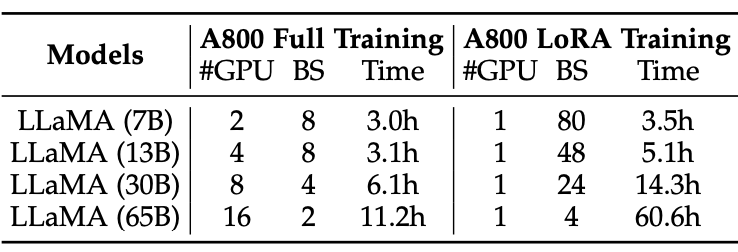
\includegraphics[width=0.99\textwidth]{fig/zhao_2023_tab7}
\caption{Training time for fine-tuning Llama}
\end{figure}

\end{frame}




\begin{frame}{Alignment tuning}

% Aligning p 4 in Zhao

\begin{itemize}
\item Problems in LLMs: fabricating false information, producing harmful, misleading, and biased expressions
% LLM may sometimes exhibit unintended behaviors, e.g., fabricating false information, pursuing inaccurate objectives, and producing harmful, misleading, and biased expressions [61, 293].
\item Similar to instruction training, but require different criterias
% However, unlike the original pre-training and adaptation tuning (e.g., instruction tuning), such an alignment requires considering very different crite- ria (e.g., helpfulness, honesty, and harmlessness).
\item The three Hs: helpfulness, honesty, and harmlessness
\item Alignment might harm the general abilities of LLMs to some extent: \uured{alignment tax}%, which is called alignment tax in related literature [295].
\item \uured{Red teaming}: Probe LLMs in an adversarial way to generate harmful outputs and then updates LLMs to prevent such outputs.

\end{itemize}

\end{frame}


\begin{frame}{Alignment tuning: Criterias}

% Aligning p 4 in Zhao
% RLHF

\begin{itemize}
\item Helpfulness
\begin{itemize}
\item To be helpful, the LLM should demon- strate a clear attempt to assist users in solving their tasks or answering questions in a concise and efficient manner as possible.
\end{itemize}
\item Honesty
\begin{itemize}
\item A LLM aligned to be honest should present accurate content to users instead of fabricating information. Additionally, it is crucial for the LLM to convey appropriate degrees of uncertainty in its output, in order to avoid any form of deception or misrepresentation of information. This requires the model to know about its capabilities and levels of knowledge (e.g., “know unknowns”).
\end{itemize}
\item Harmlessness
\begin{itemize}
\item To be harmless, it requires that the language produced by the model should not be offensive or discriminatory. To the best of its abilities, the model should be capable of detecting covert endeavors aimed at soliciting requests for malicious purposes.
\end{itemize}
\end{itemize}

\end{frame}


\begin{frame}{Alignment tuning: Human feedback}

\begin{itemize}
\item High-quality human feedback is extremely important for aligning LLMs with human pref- erences and values.
\item Human Labeler Selection. In existing work, the dominant method for generating human feedback data is human annotation. usually native speakers.
\item Three ways to collect feedback from humans:
\begin{enumerate}
\item Ranking based (choosing the best out of many suggestions)
\item Answering question about the model output (multiple choice)
\item Collect data about if the model is "breaking the rules" helpful, correct, and harmless. (as scores)
\end{enumerate}
\end{itemize}

\end{frame}


\begin{frame}{Reinforcement learning with human feedback (RLHF)}

% (discussed in Section 5.2.3)
The RLHF system mainly comprises three key components: a pre-trained LM to be aligned, a reward model learning from human feedback, and a RL algorithm training the LM.

Further, the reward model (RM) provides (learned) guidance signals that reflect human preferences for the text generated by the LM, usually in the form of a scalar value. The reward model can take on two forms: a fine-tuned LM or a LM trained de novo using human preference data.

This task would be completed step by step. At each step, an agent (i.e., LLM) will perform an action (i.e., generating a token) according to the policy (i.e., the generative probability distribution of LLM) conditioned on the current state (currently generated token sequence and other available context information)


\end{frame}


\begin{frame}{RLHF}

Three steps:
Supervised finetuning %To make the LM initially perform desired behaviors, it usually needs to collect a supervised dataset containing input prompts (instruction) and desired outputs for fine-tuning the LM.
Learn reward model: OpenAI uses 6B GPT-3 and DeepMind uses 7B Gopher
Fine-tune with the reward model

\begin{figure}[h]
\centering
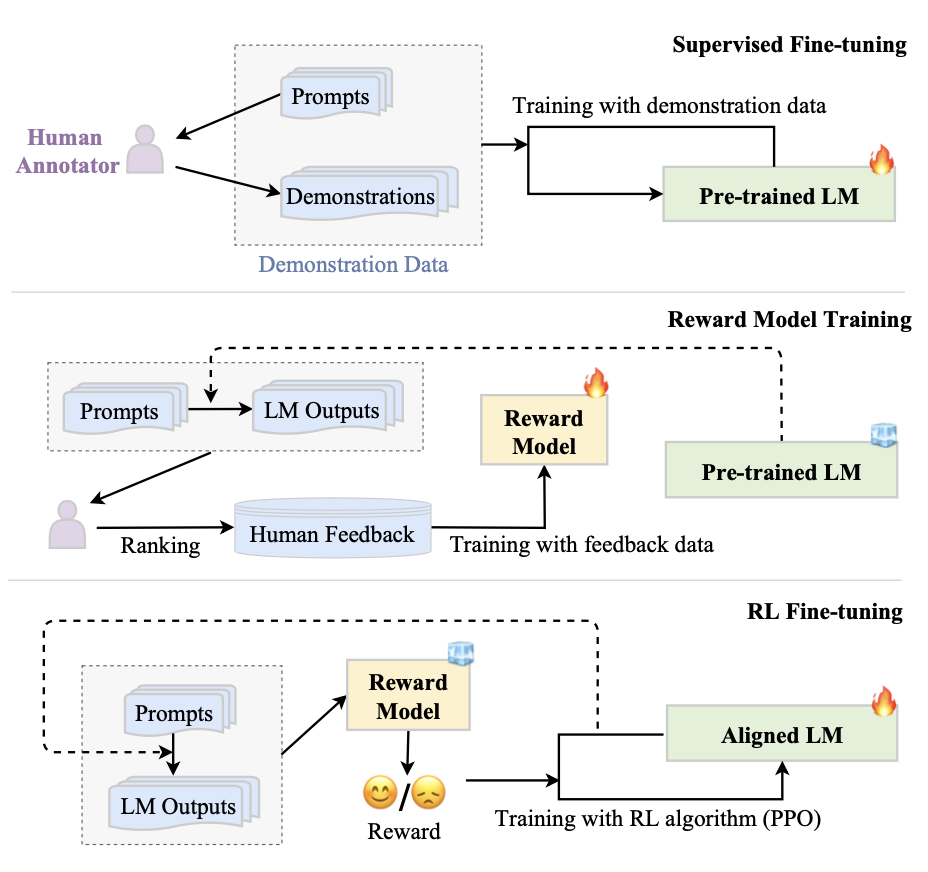
\includegraphics[width=0.99\textwidth]{fig/zhao_2023_fig10}
\caption{RLHF (Zhao, 2023, Figure 10)}
\end{figure}

\end{frame}



\begin{frame}{Hallucinations}

% Zhao
% Hallucinations
% Kaddour (2023): 2.8, Fig 7


%
% Hallucinations

\end{frame}

\section{Architectures}

\begin{frame}{GPT-3}


\end{frame}

\begin{frame}{GPT-3.5/4}


\end{frame}

\begin{frame}{Llama 2}


\end{frame}


\begin{frame}{Others}

% Table

\end{frame}


\begin{frame}{Parameters and Model Size}

% Parameters and Model Size: Use Table 1

% Uset table 3 here from Zhao


\end{frame}


\begin{frame}{Decoding (word generation)}

% Decoding (4.2.4) - sampling and temperature sampling


\end{frame}



\section{Training}

\begin{frame}{(Pre-training) Data}

% 1. Data Collection
% use Table 2 Zhao p 11 and part 4.1
% Use Figure 5 here
% Quality filtering: p 14

\end{frame}

\begin{frame}{Huge Data}

% Kaddour (2023): Unfathomable datasets - what do we do.
% Kaddour (2023): Table 1

\end{frame}

\begin{frame}{Tokenization}

% Tokenization p 15

\end{frame}

\begin{frame}{Pretraining task/Loss}

% Pretraining tasks (4.2.3)
%% Kaddour (2023): Figure 3

\end{frame}

\begin{frame}{Optimization}

% 3. Pre-Training Strategies

% Optimization - batch sizes, lr, optimizer adam p 23

% Weight decay, gradient clipping dropout p 23

\end{frame}



\section{Domain adaptation}

\begin{frame}{Domain adaptation}

% Fine tuning 5.1
% Table 7. p 28
% Kaddour (2023): 2.4


\end{frame}


\begin{frame}{Alignment tuning}

% Alignment tuning 5.2
% Helpful, harmless, honest



\end{frame}

\begin{frame}{LoRA}

% Parameter efficient fine tuning - LoRA

\end{frame}


\begin{frame}{RLHF}

% RLHF
% Table 7. p 28
% Kaddour (2023): 2.9

\end{frame}

\begin{frame}{The values of LLMs}

% Hennrich results
% Language use compared to humasn

\end{frame}


\section{Usage}

\begin{frame}{Text Generation}
% Kaddour (2023): 3.3

% Describe temperature and

\end{frame}

\begin{frame}{Code Generation}
% Kaddour (2023): 3.3


\end{frame}

\begin{frame}{Text classification}

% The results from Etienne

\end{frame}

% Kaddour (2023): 3.3

\begin{frame}{ChatBots}

% Kaddour (2023): 3.1
%C. Conversational Agents
%1. Chatbots
%2. Virtual Assistants

\end{frame}


\begin{frame}{Law and Generative (AI)}

% Law and AI: 3.6

\end{frame}



% The values of LLMs

\subsection{Prompt engineering}

\begin{frame}{How to prompt}

% take a deep breth and think.
% section 8 Zhao

\end{frame}

\section{Safety and Risks}

\begin{frame}{Risks}

% 1177 chatbot
% See Zhao

\end{frame}

\section{Future work}
\begin{frame}{Future work}

% Kaddour (2023): 2.14 unsolvable tasks?

\end{frame}



\end{document}
